% ======================================================= %
%                       Introduction                      %
% ======================================================= %
\section{Background}

    % --------------------------------------------------- %
    %                  Motivation:Goals                   %
    % --------------------------------------------------- %
    \subsection{Motivation}
    \begin{frame}{Goals}
        Aim to assess, predict, and physically explain observed two-phase flow behavior in a natural circulation loop
        \begin{Itemize}
            \item{Using a non-ideal equation of state for water}
            \item{Several models for convection and friction}
            \item{Multiple risers (non-simple loops)}
        \end{Itemize}
    \end{frame}
    
    % --------------------------------------------------- %
    %             Motivation:Leading Questions            %
    % --------------------------------------------------- %
    \begin{frame}{Leading Questions}
        \begin{Itemize}
            \item<1->{What are two-phase instabilities?}
            \begin{beamercolorbox}[sep=0.4em,rounded=true]{titlelike}
                Transient (possibly oscillatory) thermal hydraulic phenomenon stemming from 
                nonlinear-geometric-multiphase feedback that could lead to system excursions 
                causing dangerous mechanical or thermal damage and possibly human harm.
            \end{beamercolorbox}
            \pause
            \item<2->{Applications?}
                \begin{Itemize}
                    \item<2->{Thermosiphon}
                    \item<2->{Power cycle loops}
                    \item<2->{And... }
                 \end{Itemize}
        \end{Itemize}
    \end{frame}

    % --------------------------------------------------- %
    %                 RCCS:Overview                       %
    % --------------------------------------------------- %
    \subsection{RCCS}
    \begin{frame}{Reactor Cavity Cooling System}
        \begin{columns}
            \begin{column}[T]{0.45\textwidth}
                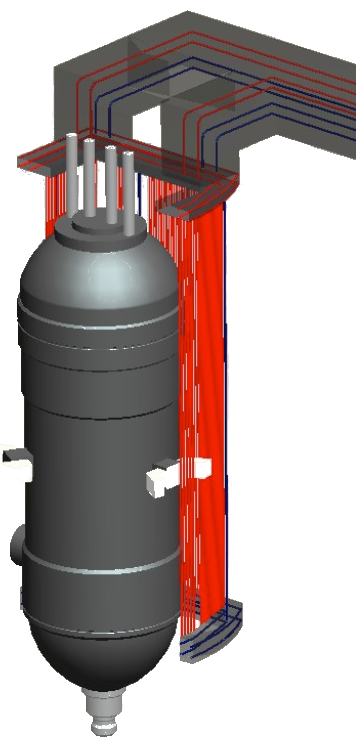
\includegraphics[height=2.5in]{RCCSMockup}
            \end{column}
            \begin{column}[T]{0.45\textwidth}
                \textbf{Purpose:}\hfill\\
                Naturally-driven cooling of reactor under accident conditions
                
                \vspace*{2em}
                \textbf{Accident conditions:}\hfill\\
                Loss of onsite, offsite power (station blackout)
            \end{column}
        \end{columns}
    \end{frame}
    

    \begin{frame}{Reactor Cavity Cooling System: Big picture}
    \begin{columns}<1>
        \begin{column}[T]{0.45\textwidth}
            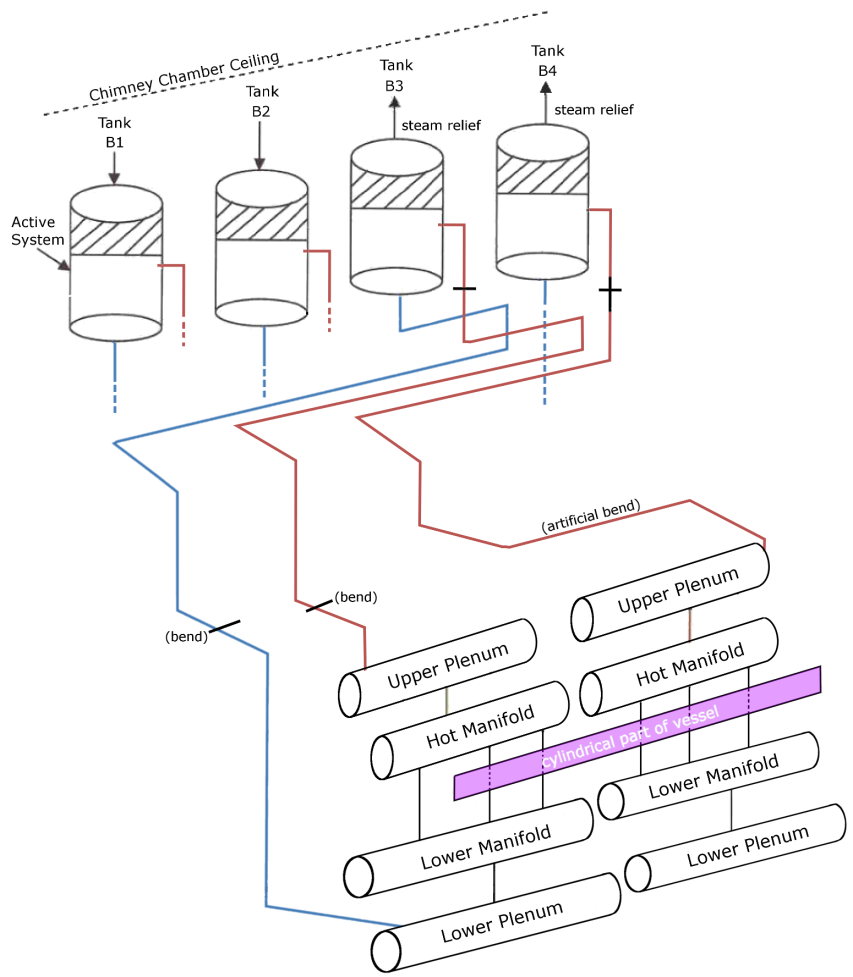
\includegraphics[height=2.5in]{RCCSTotalSystem}
        \end{column}
         \begin{column}[T]{0.45\textwidth}
            \textbf{Selected specifications:}\\[0.2em]
            \begin{Itemize}
                \item{Trains: 2}
                \item{Lines/Tanks: 8}
                \item{Elevation change: 35 meters}
                \item{Path length: 200 meters}
                \item{Heated length: 20 meters}
                \item{Risers: 200+}
                \item{Heat transfer:}
                \begin{Itemize}
                    \item{Radiation: 80\%}
                    \item{Convection: 20\%}
                \end{Itemize}
            \end{Itemize}
        \end{column}
    \end{columns}
\end{frame}


    % --------------------------------------------------- %
    %                 RCCS:Experiment                     %
    % --------------------------------------------------- %
    \begin{frame}[c]{RCCS Experiment}
        \begin{columns}[c]
            \begin{column}{0.35\textwidth}
                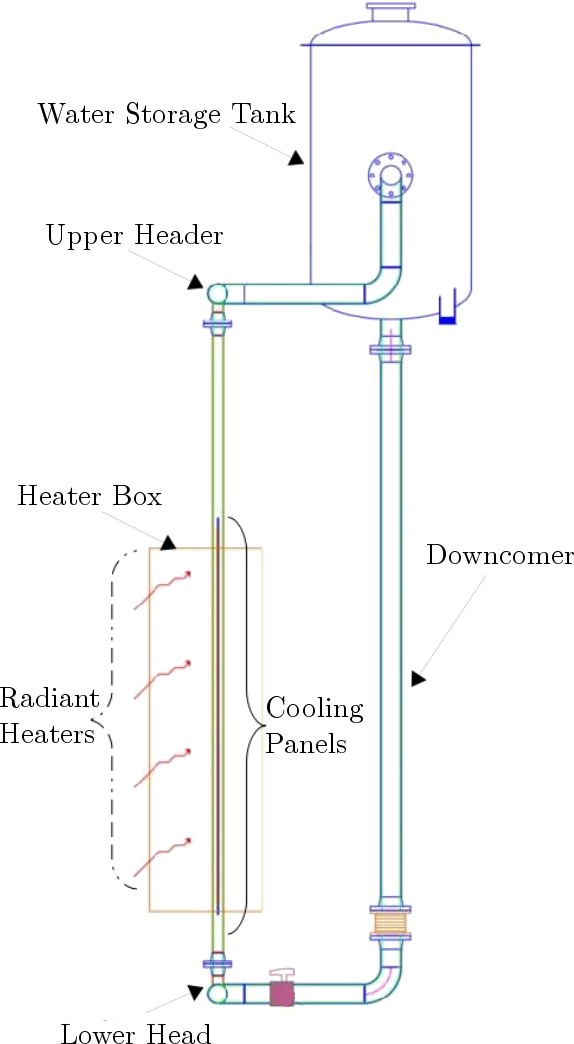
\includegraphics[height=2.5in]{RCCSExperimentOverview}
            \end{column}
            \begin{column}{0.60\textwidth}
                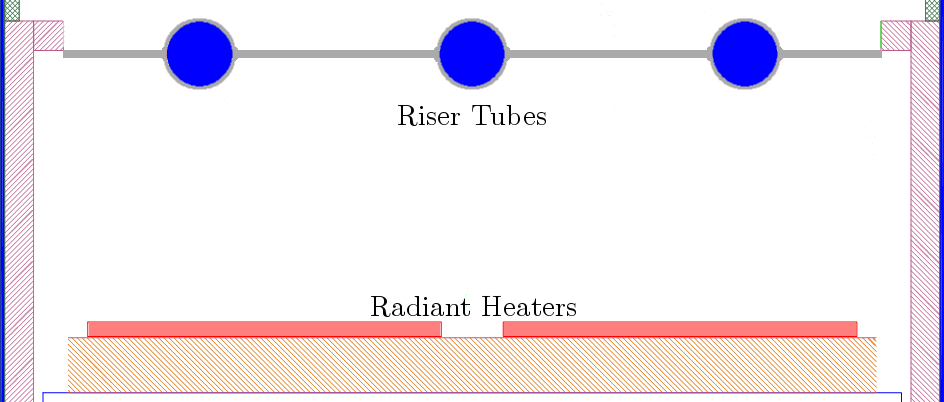
\includegraphics[width=2.5in,angle=0]{RCCSExperimentHeatBox}
            \end{column}
        \end{columns}
    \end{frame}
    
    
    
    % --------------------------------------------------- %
    %                 RCCS:Mass Flow rate                 %
    % --------------------------------------------------- %
    \begin{frame}[c]{Experimental data: flow oscillations during boiling}
        \begin{center}
            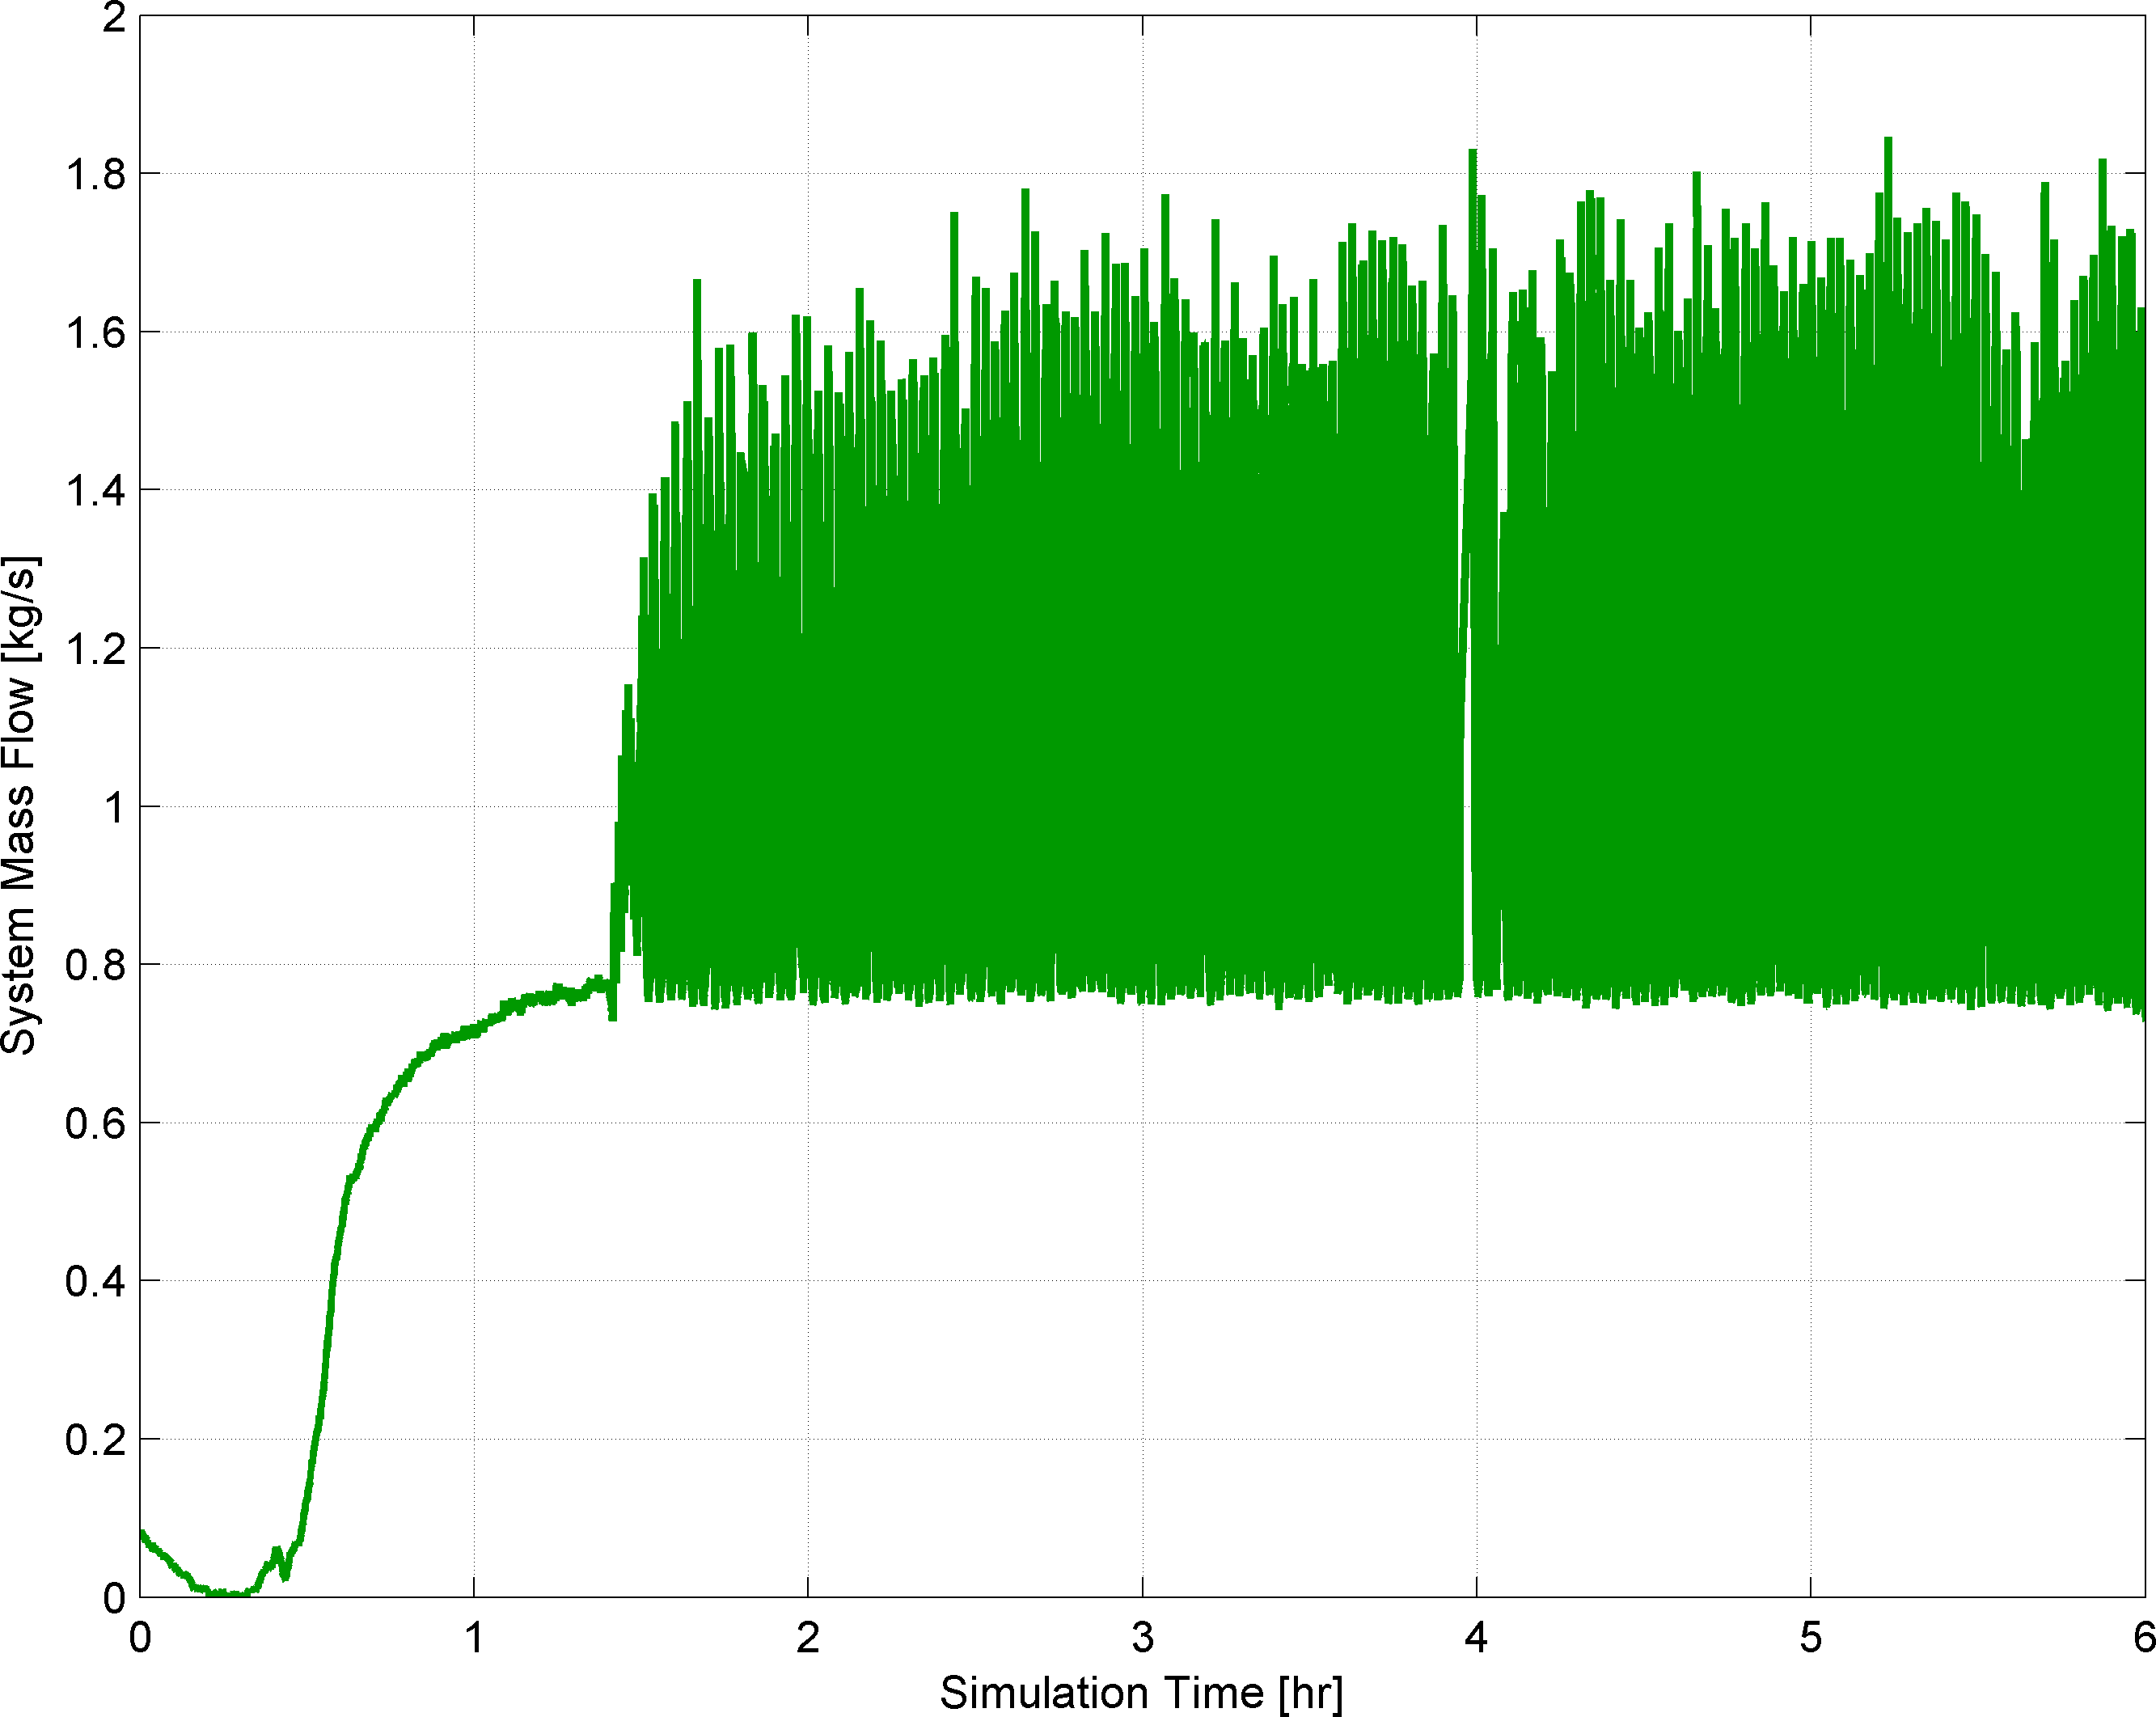
\includegraphics[height=2.5in]{ExperimentMassFlow}
        \end{center}
    \end{frame}



    % --------------------------------------------------- %
    %                     Literature                      %
    % --------------------------------------------------- %
    \subsection{Literature}
    \begin{frame}{Been done before?}
        Two-phase, natural circulation stability literature exists.
        \vspace{1em}
        But...
        \begin{Itemize}
            \item{Almost no analytical work on non-simple, closed loop (multiple riser)}
            \item{None had depletion of inventory in two-phase}
        \end{Itemize}
    \end{frame}
